%* 
%* ------------------------------------------------------------------
%* DispatcherReference.tex - Dispatcher Reference
%* Created by Robert Heller on Wed May 28 18:01:28 2008
%* ------------------------------------------------------------------
%* Modification History: $Log$
%* Modification History: Revision 1.1  2002/07/28 14:03:50  heller
%* Modification History: Add it copyright notice headers
%* Modification History:
%* ------------------------------------------------------------------
%* Contents:
%* ------------------------------------------------------------------
%*  
%*     Model RR System, Version 2
%*     Copyright (C) 1994,1995,2002-2005  Robert Heller D/B/A Deepwoods Software
%* 			51 Locke Hill Road
%* 			Wendell, MA 01379-9728
%* 
%*     This program is free software; you can redistribute it and/or modify
%*     it under the terms of the GNU General Public License as published by
%*     the Free Software Foundation; either version 2 of the License, or
%*     (at your option) any later version.
%* 
%*     This program is distributed in the hope that it will be useful,
%*     but WITHOUT ANY WARRANTY; without even the implied warranty of
%*     MERCHANTABILITY or FITNESS FOR A PARTICULAR PURPOSE.  See the
%*     GNU General Public License for more details.
%* 
%*     You should have received a copy of the GNU General Public License
%*     along with this program; if not, write to the Free Software
%*     Foundation, Inc., 675 Mass Ave, Cambridge, MA 02139, USA.
%* 
%*  
%* 


\chapter{Dispatcher Reference}
\label{chpt:dispatcher:Reference}
\typeout{$Id$}

The Dispatcher program is used to create computerized CTC (Centralized
Traffic Control) panels, to be used by dispatchers as part of a CATC
(Computer Assisted Traffic Control) system to manage traffic flow for a
model railroad.  A computerized CTC panel typically contains a track work
schematic and a collection of control elements (such as switch plates,
signal plates, toggle switches, push buttons, etc.) that control the
track work and track side signals.  In addition to creating and editing
CTC panels, the Dispatcher program can read in an XTrkCAD layout file
and create a compressed graph of the track work and this graph can be
used as a guide while creating CTC panels.

\section{Main GUI Screen}

\begin{figure}[hbpt]
\begin{centering}
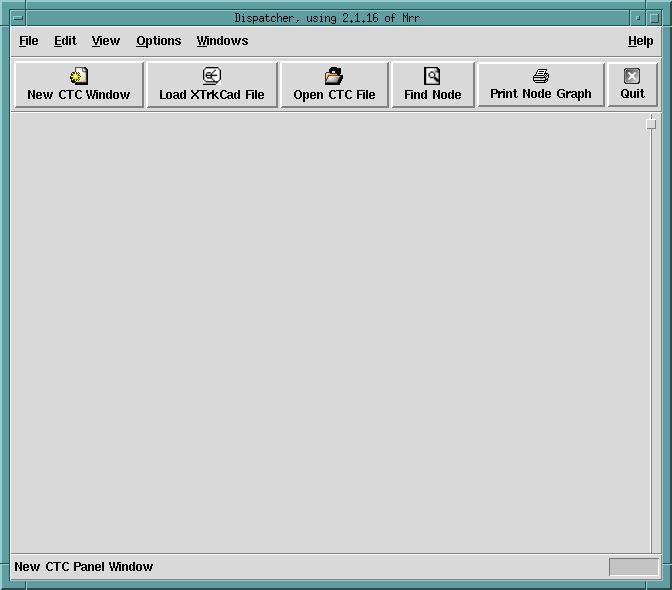
\includegraphics[width=5in]{DISPMainGUI.png}
\caption{Main Dispatcher Window}
\label{fig:dispatcher:mainDispatcher}
\end{centering}
\end{figure}
The main GUI window of the Dispatcher program is shown in
Figure~\ref{fig:dispatcher:mainDispatcher}. It consists of a standard
menu bar, a tool bar, and an area for track work graph display. A
track work graph is something computer scientists call a ``directed
graph''.  A directed graph is a data structure consisting of nodes,
with links to other nodes.  In this case each node is a piece of
track work and the links are the connections between pieces of track work
and thus indicate the adjacency of track work nodes (and how the pieces
of track work interconnect with each other).  In the case of simple
track work (such as straight sections or curved sections), there are one
(if the section ``dead ends'') or two links and in the case of complex
track work (such as turnouts and crossings), there are three or more
links.  The graph is ``compressed'', where adjacent pieces of simple
track work are consolidated into single nodes. 

\subsection{Track work Node Graphs}

Once the compressed graph is built (upon loading a layout file), it is
displayed on the main GUI screen as numbered circles (nodes) connected
by lines with arrows (links).  A graphic of the piece of track work is
also drawn. Left clicking on a node displays a pop-up containing
information about the track work node.  Right clicking on a node pops up
a menu of actions involving the node\footnote{Current two menu items
are defined, one to display the node info and the other to add it to a
panel.}. Left clicking on a link displays a pop-up containing
information about the link.  The node numbers are the track element
numbers assigned by XTrkCad.

\subsubsection{Loading a Layout}

An XTrkCAD layout file is loaded either with the \verb=Load XTrkCad File=
tool bar button or with the \verb=Load...= item on the \verb=File=
menu. It is also possible to load a XTrkCAD layout file during
program startup using the \verb=-xtrkcad= command line option.

In all cases, the layout's track work is loaded a track work graph and
displayed in the track work graph display area.  Dispatcher then asks if
XTrkCad itself should be started.  This might be useful as it gives a
display of the actual layout on your screen, which can be referred to
when creating CTC panels.

\subsubsection{Finding Nodes}

A node can be ``found'' by its number.  Finding a node scrolls the node
graph to make the node visible and the node is highlighted.

\subsubsection{Printing Node Graphs}

A node graph can be printed to provide a hard-copy reference of the node
graph.

\subsection{Creating a new CTC Panel}
\label{sect:dispatcher:creatingCTCPanels}

\begin{figure}[hbpt]
\begin{centering}
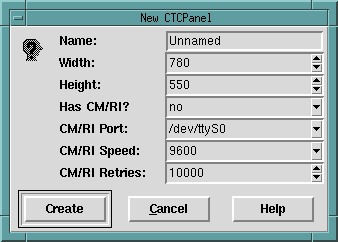
\includegraphics{DISPNewCTCPanel.png}
\caption{New CTC Panel Dialog}
\label{fig:dispatcher:newCTCPanel}
\end{centering}
\end{figure}
A new CTC Panel is created with the \verb=New CTC Window= too bar button or
the \verb=New CTC Panel Window= entry under the \verb=File= menu.  A New
CTC Panel Dialog, as shown in Figure~\ref{fig:dispatcher:newCTCPanel}, is
displayed. This dialog box asks the user for some basic information
about the new panel.  This includes the name (title) of the panel, its
initial width and height, whether it connects to a C/MRI bus and
information about that bus.

What is actually created is a Tcl/Tk program that uses parts of the
library of Tcl/Tk and C++ code included with the Model Railroad System
that will implement a CTC Panel, which contains two display sections: a
track work schematic and a control panel.  The track work schematic is in
the upper half of the panel and has a black background with white (red
when occupied) track work. Signals with one, two, or three heads can be
added to the track work schematic.  The control panel is in the lower
half and has a dark green background. The control panel can have switch
plates, signal plates, toggle switches, push buttons, code buttons, and
indicator lamps.

The CTC Panel can be used by a dispatcher using a computer screen and
pointing device (such as a mouse or touch pad) to select and manipulate
control elements. The track work on a CTC Panel will reflect the actual
track conditions (occupied or not, signal aspects, and turnout states).

\subsection{Opening an existing CTC Panel}

Existing CTC Panel programs are the specifically formatted Tcl/Tk programs
created by the Dispatcher program.  They can be opened and edited using
the \verb=Open CTC File= too bar button or the \verb=Open...= entry under
the \verb=File= menu or specified on the Dispatcher's command line. 
There are three sections of the code that are ``loaded'' into the
Dispatcher program: the collection of CTC Panel elements, the
information about the (optional) C/MRI network, and the user code
associated with the panel.

\section{Configurable Options}
\label{sect:dispatcher:configopts}

The configurable options can be set or changed with the 
\verb=Edit Configuration= menu entry under the \verb=Options= menu. These
configurable options can be saved with the \verb=Save Configuration=
menu entry under the \verb=Options= menu and can be loaded with the 
\verb=Load Configuration= menu entry.  At present there are two
configuration options: \verb=Use External Editor=, which has a boolean
value (true or false) and \verb=External Editor=, which is a
command line that starts an external editor (the name of the file
to edit is appended to this command line).

\section{CTC Panel Windows}

\begin{figure}[hbpt]
\begin{centering}
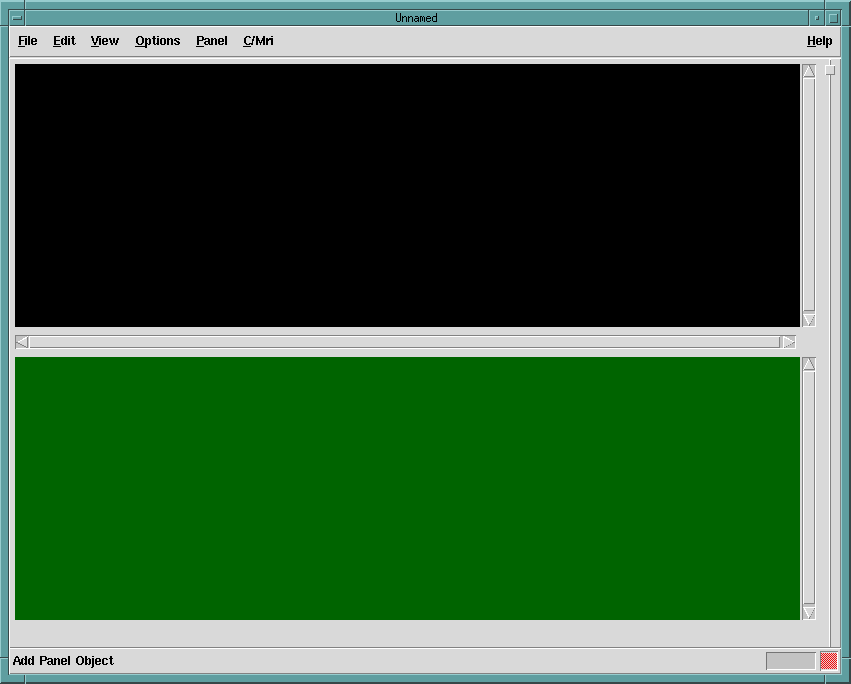
\includegraphics[width=5in]{DISPEmptyCTCPanel.png}
\caption{Empty CTC Panel Window}
\label{fig:dispatcher:emptyCTCPanel}
\end{centering}
\end{figure}
A freshly created CTC Panel window is shown in
Figure~\ref{fig:dispatcher:emptyCTCPanel}\footnote{When the program is
run on its own, the Panel and C/Mri menus will be absent.}. The pink
square at the lower left indicates that the file is in a modified state
and has not been saved to disk.  Saving the file is done with the
\verb=Save= and \verb=Save As...= menu items under the \verb=File= menu.

\subsection{Menu items available when editing a CTC Panel Window}

\subsubsection{File menu}

The \verb=File= contains entries to create a new CTC Panel Window, load
an XTrkCad file, open a CTC Panel Window, save the current CTC Panel
Window, close the current CTC Panel Window, and exit.  Attempting to
close a modified CTC Panel Window will cause a save confirmation window,
allowing you to save your work.

\subsubsection{Edit menu}

In addition to the standard edit menu entries, there are three extra
entries:

\begin{description}
  \item[(Re-)Generate Main Loop] This entry generates (or regenerates)
the main loop.  The basic loop read all of the input ports of all of the
C/MRI nodes, invokes all of the track work elements, and then writes all
of the output ports of all of the C/MRI nodes.  The loop is an endless
real time loop.  It is necessary to ``fill in'' the logic of the CTC Panel.
  \item[User Code] This entry opens an editor to edit the user code
section of the CTC Panel program.
  \item[Modules] This entry inserts selected helper modules into the
user code section of the CTC Panel program.  These are all in namespaces
and are SNIT types:
    \begin{description}
      \item[Track Work types] This inserts two SNIT types, one for
blocks (usable for simple track work) and one for switches (turnouts).
      \item[Switch Plate type] This inserts a SNIT type to handle switch
plates. 
      \item[Signals] This inserts SNIT types to help with signals:
	\begin{description}
	   \item[Two Aspect Color Light] Use this module if you are
using two lamp or LED (red and green) signals.  One, two, and three head
signals are supported.
	   \item[Three Aspect Color Light] Use this module if you are
using three  lamp or LED (red,  yellow,  and green) signals.  One, two,
and three head signals are supported.
	   \item[Three Aspect Search Light] Use this module if you are 
using bi-color LEDs (red/green -- either three lead or two lead)
signals.  One, two, and three head signals are supported.
	\end{description}
      \item[Signal Plate type] This type handles Signal Plates.
      \item[Control Point type] Use this type for Code Button action code.
      \item[Radio Group Type] Use this type to collect a group of push 
buttons into an exclusive group where only one button is ``on'' at a
time.  Used to implement a software track selection matrix for a yard or
terminal.
    \end{description}
\end{description}

\subsubsection{View menu}

The \verb=View= menu contains entries to zoom in, zoom to a specific
level, and zoom out. This allows to grow or shrink the display.  This
lets the dispatcher get a view of a large layout in a single view or to
zoom in on a specific control point as needed.  This menu is also
available in the generated CTC Panel program.

\subsubsection{Panel menu}

The \verb=Panel= menu contains entries to add, edit, and delete panel
elements (both track work and control) and also has an entry to edit the
overall panel's configuration. 

\subsubsection{C/Mri menu}

The \verb=C/Mri= menu contains entries to add, edit, and delete C/MRI
nodes on the C/MRI bus. The C/MRI nodes contain input and output ports
that can be connected to things like occupancy detectors, turnout point
state switches, signal LEDs (or lamps), and switch machine motors.  They
can also be connected to manual controls and indicators on control
panels mounted over on beside the layout (eg ``local'' towers).


\section{CTC Panel Code}

The Dispatcher program creates Tcl scripts (programs).  That is, each
CTC Panel Window implies a Tcl/Tk script file and in fact this is what
is created when the window is ``saved''.  The script file contains
generated code, code that is created by the Dispatcher program (some of
which is pre-written code that is copied to the script file). And some
of the code is created by you the user of the program. This code
implements the CTC Panel that your model railroad's dispatcher will use
to control some part of your model railroad during an operating session.

\subsection{Generated Code}

The generated code consists of some prefix code including comments
containing the panel's configuration, followed by code to load various
packages used by the CTC Panel code, code to implement the panel
itself, and code to initialize the C/MRI bus and initialize the nodes
(boards) on the bus.

\subsubsection{Configuring CTC Panel Windows}

\begin{figure}[hbpt]
\begin{centering}
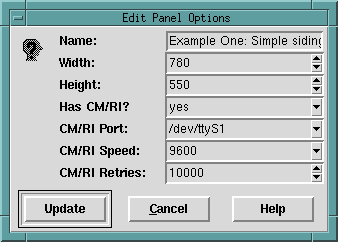
\includegraphics{DISPEditPanelOptions.png}
\caption{Edit Panel Options Dialog}
\label{fig:dispatcher:editPanelOptsDialog}
\end{centering}
\end{figure}
The configuration of CTC Panel Windows can be changed using the
\verb=Configure= entry of the \verb=Panel= menu.  This menu entry
displays the Edit Panel Options Dialog, as shown in
Figure~\ref{fig:dispatcher:editPanelOptsDialog}. This dialog box allows
changing all of the same options as were set when the panel was created
(see Section~\ref{sect:dispatcher:creatingCTCPanels}).

\subsubsection{Adding, Editing, and deleting elements to CTC Panel Windows}

CTC Panel elements can be added, edited, or deleted with the
\verb=Add=, \verb=Edit=, and \verb=Delete= entries of the \verb=Panel=
menu. There are twenty element types to select from.  CTC Panel
trackwork elements can also be added directly from the Track work Node
Graphs using the right button node menu.  Every CTC Panel element has a
unique name, is part of a control point\footnote{For mainline trackage a
control point of ``Main'' can be used.}, and has an X, Y location on
either the trackwork schematic or the control area. Additionally,
element specific options are available for each element.

\subsubsection{Adding, Editing, and deleting C/Mri nodes to CTC Panel
Windows}

C/Mri nodes can be added, edited, or deleted with the \verb=Add=,
\verb=Edit=, and \verb=Delete= entries of the \verb=C/Mri=menu. Each
node has a unique name and unique UA (address).  There are three
supported board types: SMINI (Super Mini), USIC (Universal Serial
Interface Card) and SUSIC (Super Universal Serial Interface Card).

\subsection{User Code}

The user code is editable with the \verb=User Code= entry of the
\verb=Edit= menu.  This menu entry either starts a simple edit window or
starts a user-specified external editor (See
Section~\ref{sect:dispatcher:configopts}).  In addition to directly
editing the user code, one or more pre-written modules can be inserted
and a skeleton main loop can be created.

\subsubsection{Insertable Modules}

These are a collection of SNIT types, in namespaces, that encapsulate
various common types of things that a CTC Panel implements, including
blocks, turnouts, signals, signal plates, control points, and radio
groups (commonly used to implement a software track selection matrix for
a yard or terminal).

\subsubsection{The Main Loop}

A skeleton main loop can be generated, but you will need to modify it to
implement the actual logic of your CTC Panels.  The basic main loop is an
endless, ``real time'' loop, that reads in all of the input ports,
invokes all of the trackwork, and then writes all of the output ports. 
It is necessary to decode the input bytes into bit fields which can be
stored in various types.  The occupation state and switch point state
information sensed from the inputs is used, along with the settings of
the control elements (switch plates, signal plates, etc.) is tested and
logical tests are applied to determine things like signal aspects and
switch motor values, etc. These values are then packed into the vectors
(lists) of output bytes which are then written to the output ports.

